\documentclass[12pt,a4paper]{article}
\usepackage[T1]{fontenc}
\usepackage{amsmath}
\usepackage{amsfonts}
\usepackage{amssymb}
\usepackage{graphicx}
\usepackage{inputenc}
\usepackage[bottom=1.5cm]{geometry}
\usepackage{lscape}
\usepackage{booktabs}
\usepackage{multirow}
\usepackage[table,xcdraw]{xcolor}
\usepackage{tikz}
\usetikzlibrary{shapes}
\usetikzlibrary{trees}
%\renewcommand\seriesdefault{bx}
%\usepackage{bold-extra}

\begin{document}
  
  {
   \setlength{\topmargin}{-2cm}
   \enlargethispage{30mm}
\begin{titlepage}
  \begin{center}
    
	\begin{figure}[h]
    \centering
    \begin{minipage}{.45\textwidth}
    \centering
    \includegraphics[width=.7\linewidth]{../figures/logoBE.png}
    \end{minipage}%
    \begin{minipage}{.45\textwidth}
    \centering
    
\includegraphics[height=.7\linewidth]{../figures/UNDP-LOGO.pdf}
    \end{minipage}
    \end{figure}    
    
    
   \vspace{0.5cm}

        {\sc 
\includegraphics[width=0.36\textwidth, height=0.14\textwidth]{../figures/LOGO EEIA.png}}\\[1em]
        {\sc {}}
    
        \vspace{1.2cm}
    \centerline{\hbox to 13cm{\hrulefill}}
    \vspace{0.3cm}
    { \Large  \uppercase{\textbf{{Syllabus de la semaine\\ de Machine Learning }}}}
    \vspace{0.3cm}
    \centerline{\hbox to 13cm{\hrulefill}}
    
    \vspace{1.2cm}
    {\sc \Large {Par l'équipe pédagogique}\\ [1.5 cm]
    %\large Supervisor: \\ [0.2 cm]
    %        \large Prof. Name Surname \\ [0.2 cm]
    %        \large University of Somewhere
    }
    \vspace{1.7cm}
    
   \begin{figure}[h]
    \centering
    \begin{minipage}{.45\textwidth}
    \centering
    
\includegraphics[width=.7\linewidth]{../figures/logoFV.jpg}
    \end{minipage}%
    \begin{minipage}{.45\textwidth}
    \centering
    
\includegraphics[width=.7\linewidth]{../figures/Fondation_de_France.png}
    \end{minipage}
    \end{figure}
    
    \vspace{0.5cm}
    

    
    \hbox to \textwidth{\hrulefill}
    \vspace{0.2cm}
    {\sc  EDITION 2025 - Version Draft}
    
  \end{center}
\end{titlepage}
}
\section{Introduction}

L’introduction de l’apprentissage automatique (Machine Learning) s’étale sur 6 jours. Durant cette semaine, les apprenants vont construire différents modèles prédictifs, comprendre les types de problèmes dans lesquels ils peuvent être utilisés et interpréter le résultat de ces modèles (éventuellement, ses paramètres).
De plus, l’équipe d’enseignants s’assurera que les élèves se familiarisent avec le processus de développement de modèles de la définition d’un problème à la maintenance du modèle.
En somme, les objectifs de la semaine, telle que décrite dans les sections suivantes, sont:
\begin{enumerate}
\item Les élèves sont capables, étant donné une base de donnée et connaissant la typologie du modèle (régression linéaire, k-means, régression logistique, arbre de décision, réseaux de neurones\dots{}) voulu, de calibrer le modèle avec du code Python;

\item Les élèves sont capables, étant donné une base de donnée et un problème défini, de donner une proposition de modèle qui serait le plus adapté pour résoudre le problème, en justifiant leur choix à partir des caractéristiques des données (quantité, nature des variables, etc.) et des objectifs du projet;

\item Les élèves sont capables d'interpréter les paramètres des modèles qui en possèdent et de faire des prédictions avec Python;

\item Les élèves sont familiers avec les différentes étapes d’un projet de développement de modèle, ont un premier contact avec les principaux concepts et sont capables d’expliquer l’intérêt de chacune de ces étapes.
\end{enumerate}

\section{Emploi du temps}

% Please add the following required packages to your document preamble:
% \usepackage{booktabs}
% \usepackage{multirow}
% \usepackage{graphicx}
% \usepackage[table,xcdraw]{xcolor}
% Beamer presentation requires \usepackage{colortbl} instead of \usepackage[table,xcdraw]{xcolor}
% \usepackage{lscape}
\begin{landscape}
\begin{table}[]
\small
%\resizebox{\textwidth}{!}{%
\begin{tabular}{@{}lllllll@{}}
\toprule
      & Jour 1: Introduction                                                                                         & Jour 2: Classification                                                   & Jour 3: Régressions                                                                   & Jour 4: Apprentissage profond & Jour 5: Optimisation                                                                                & Jour 6: Synthèse                                                                                                               \\ \midrule
8h00  & \begin{tabular}[c]{@{}l@{}}Introduction à \\l'apprentissage statistique\\  (Espéran Padonou)\\ 3h\end{tabular} & \begin{tabular}[c]{@{}l@{}}K-means \\ (Johannès)\\ 1h30\end{tabular}                & \begin{tabular}[c]{@{}l@{}}Régression Linéaire \\ (\_\_\_) \\ 1h30\end{tabular}        &                                                                                                                           &                                                                                                     &                                                                                                                                \\
      & 30mn de pause                                                                                                & 30mn de pause                                                                       & 30 mn de pause                                                                        &                                                                                                                           &                                                                                                     & \multirow{-2}{*}{\begin{tabular}[c]{@{}l@{}}Processus \\ de développement\\ de Modèles (Part II)\\ (\_\_\_\_) \\ 2h/3h\end{tabular}} \\
      & \begin{tabular}[c]{@{}l@{}}Processus de développement\\ de Modèles (Part I)\\ 1h\end{tabular}                  & TPs K-means - 2h                                                                    & \begin{tabular}[c]{@{}l@{}}TPs de Reg. linéaire  \\ 2h   \end{tabular} & \multirow{-3}{*}{\begin{tabular}[c]{@{}l@{}}Introduction aux \\ réseaux de Neurones \\ (Syntyche/Junior) \\ 3h30\end{tabular}} & \multirow{-3}{*}{\begin{tabular}[c]{@{}l@{}}Optimisation \\ (Rodolphe Leriche) \\ 3h30\end{tabular}} &                                                                                                                                \\ \cmidrule(l){2-7} 
      &                                                                                                              &                                                                                     &                                                                                       &                                                                                                                           &                                                                                                     &                                                                                                                                \\ \midrule
14h00 & \begin{tabular}[c]{@{}l@{}}Processus de développement\\ de Modèles Part I \\ 1h\end{tabular}                 & \begin{tabular}[c]{@{}l@{}}Arbres de décision \\ (Kevin Kpakpo) - 1h30\end{tabular} & \begin{tabular}[c]{@{}l@{}}Régression Logistique\\ (Modeste Dayé) - 1h30\end{tabular} & \cellcolor[HTML]{FFFFC7}                                                                                                  & TP optimisation - 2h                                                                                &                                                                                                                                \\
      & 15mn de pause                                                                                                & 15mn de pause                                                                       & 15mn de pause                                                                         & \multirow{-2}{*}{\cellcolor[HTML]{FFFFC7}Conférence}                                                                      &                                                                                                     &                                                                                                                                \\
      & \begin{tabular}[c]{@{}l@{}}Statistique Graphique\\ (\_\_\_\_) \\ 1h30\end{tabular}                            & \begin{tabular}[c]{@{}l@{}}TPs arbres de décision \\ 2h   \end{tabular}                                                                      & TPs de logistique - 2h                                                                &                                                                                                                           &                                                                                                     &                                                                                                                                \\ \bottomrule
\end{tabular}%
%}
\end{table}
\end{landscape}

\section{Description des cours}
\subsection{Introduction à l'apprentissage statistique}

\textbf{Durée:} 3h\\
\textbf{Résumé:} Le cours donne un panorama de différentes applications dans lesquelles l’utilisation de modèles statistiques peut apporter des éléments de réponses. Il doit confronter les élèves à des problèmes concrets et les amener à définir des questions telles qu’un modèle puisse répondre à ceux-ci.\\
\textbf{Acquis du cours:} A la sortie du cours, les élèves doivent:
\begin{enumerate}
\item Connaître les catégories de problème de ML (Régression, Classification, Clustering, Réduction de dimension, Apprentissage renforcé) en définissant les termes “non-supervisé” et “supervisé”;
\item Etre capable de donner des exemples concrets de problèmes pour chacune de ces catégories;
\item Comprendre le concept d’erreur statistique: le modèle prédictif impose un type de relation qui crée une erreur qu’on cherche à minimiser (d’où l’utilité du cours d’optimisation)
\end{enumerate}


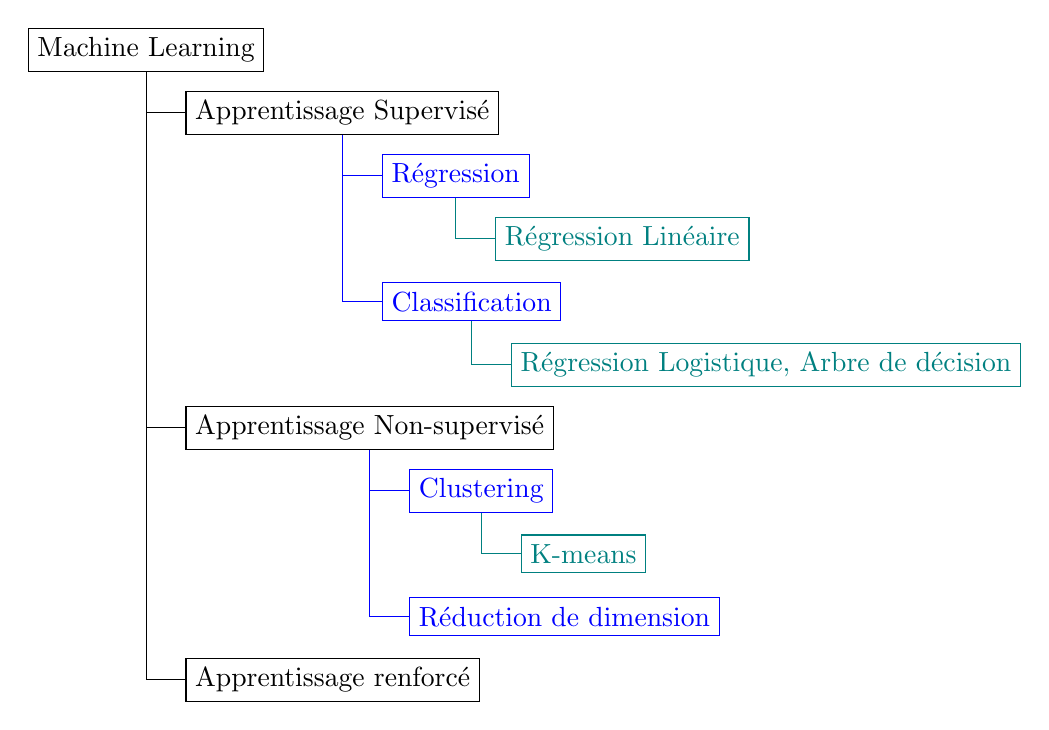
\begin{tikzpicture}
[
    level 1/.style = {black},
    level 2/.style = {blue},
    level 3/.style = {teal},
    every node/.append style = {draw, anchor = west},
    grow via three points={one child at (0.5,-0.8) and two children at (0.5,-0.8) and (0.5,-1.6)},
    edge from parent path={(\tikzparentnode\tikzparentanchor) |- (\tikzchildnode\tikzchildanchor)}]
 
\node {Machine Learning}
    child {node {Apprentissage Supervisé}
    child {node {Régression}
    child {node {Régression Linéaire}}}
    child [missing] {}
    child {node {Classification}
    child {node {Régression Logistique, Arbre de décision}}
    }} 
    child [missing] {}
    child [missing] {}
    child [missing] {}
    child [missing] {}
    child {node {Apprentissage Non-supervisé}
    child {node {Clustering}
    child {node {K-means}}}
    child [missing] {}
    child {node {Réduction de dimension}}}    
    child [missing] {}
    child [missing] {}
    child [missing] {}
    child {node {Apprentissage renforcé}};
 
\end{tikzpicture}

\subsection{Processus de développement de Modèles - Part I}

\textbf{Durée:} 2h\\
\textbf{Résumé:} Le cours présente les étapes de développement de modèles statistiques. Il se concentre sur l’aspect théorique de chaque étape et justifie leur intérêt. Il doit donner aux élèves le point de vue d’un modélisateur face à un problème: “Comment je collecte les données? Quelle est la qualité de ces données? Comment j’améliore cette qualité? (Prétraitement des données) Je ne connais pas les variables et les relations entre elles. Comment résumer rapidement ces relations? (analyse exploratoire des données) Vu les relations que j’observe, il y a-t-il un intérêt à créer de nouvelles variables? (ingénierie des caractéristiques) Comment faire pour calibrer et savoir s’il se comportera bien sur de nouvelles données? (entraînement et évaluation de modèle) Pendant que l’utilisation de ce modèle, comment je sais qu’il fait de bonnes prédictions?”\\
\textbf{Acquis du cours:} A la sortie du cours, les élèves doivent:
\begin{enumerate}
\item Connaître les étapes du processus de développement et expliquer leur intérêt;
\item Donner des exemples d’indicateurs de performance simple: RMSE, MAE,  Précision, Sensibilité;
\item Comprendre que les cours qui suivent ne décrivent que l’étape d’entraînement de modèle.
\end{enumerate}


\subsection{Statistique Graphique}

\textbf{Durée:} 1h30\\
\textbf{Résumé:} Le cours aborde une partie de la problématique de l’Analyse Exploratoire des Données. Il présente quelques graphes utilisés pour extraire des informations d’une base de données. Les élèves sont initiés aux catégories de variables (quantitatives et qualitatives). A partir de ces définitions, le cours leur donne des éléments pour décider du graphe le plus approprié suivant l’objectif voulu.\\
\textbf{Acquis du cours:} A la sortie du cours, les élèves doivent être:
\begin{enumerate}
\item capable d’expliquer l’objectif des graphes;
\item capable de classer une variable dans une catégorie (continue, discrète, ordinale, nominale);
\item capable d’interpréter une moyenne, une médiane,  un mode, l’écart type, et l’intervalle interquartile;
\item capable de décider quand utiliser un histogramme, un barplot, un graphique linéaire, nuage de points, une boîte à moustache.
\end{enumerate}



\subsection{K-means}

\textbf{Durée:} 1h30 - TD 2h\\
\textbf{Résumé:} Le cours présente l’algorithme des K-means à partir d’un exemple simple. Les élèves s’entraînent à calculer les barycentres et les distances des points à ceux-ci.\\
\textbf{Acquis du cours:} A la sortie du cours, les élèves doivent être:
\begin{enumerate}
\item Etre capable d’expliquer l’algorithme de K-means;
\item comprendre dans quels contextes ce type de modèle est conseillé;
\item Être capable de calibrer un modèle et de faire des prédictions.
\end{enumerate}

\subsection{Arbre de décision}

\textbf{Durée:} 1h30 - TD 2h\\
\textbf{Résumé:} Le cours présente un jeu qui peut être optimisé à l’aide d’un arbre de décision. A travers ce jeu, l’élève se familiarise à la structure d’un arbre. Il donne à l’élève une compréhension détaillée de l’entropie de Shannon. Elle est utilisée pour quantifier/représenter le gain d’information (réduction d’hétérogénéité).\\
\textbf{Acquis du cours:} A la sortie du cours, les élèves doivent être:
\begin{enumerate}
\item Etre capable de définir un arbre de décision et les principales notions; 
\item Comprendre les contextes (segmentation des problèmes) dans lesquels ce type de modèle est judicieux;
\item Etre capable de décrire l’algorithme de construction de l’arbre;
\item Etre capable de calibrer un modèle et de faire la prédiction;
\item Etre capable d’évaluer le modèle;
\item (optionnel) citer les inconvénients de l’arbre de décision et présenter la forêt aléatoire.
\end{enumerate}

\subsection{Régression Linéaire}

\textbf{Durée:} 1h30 - TD 2h\\
\textbf{Résumé:} le cours implémente une régression linéaire pour modéliser la consommation de poulet avec la population des pays africains. \\
\textbf{Acquis du cours:} A la sortie du cours, les élèves doivent:
\begin{enumerate}
\item Etre capable de définir la régression linéaire (et les principaux termes: coefficients, ordonnée à l’origine); 
\item Être capable de donner des exemples pour lesquels, calibrer une régression linéaire est possible;
\item Etre capable de calibrer le modèle et comprendre l’interprétation des paramètres;
\item Être conscient du risque d’intégrer des valeurs extrêmes dans les données de calibration;
\item Comprendre le lien entre la calibration et l’optimisation.
\end{enumerate}

\subsection{Régression Logistique}

\textbf{Durée:} 1h30 - TD 2h\\
\textbf{Résumé:} Comme exemple de méthode de classification, la régression logistique est présentée dans ce cours à travers une étude de cas simple. Il guidera l’élève pour prédire le mode de transport choisi suivant les conditions météorologiques et de circulation. \\
\textbf{Acquis du cours:} A la sortie du cours, les élèves doivent:
\begin{enumerate}
\item Etre capable de définir la régression logistique (coefficients, formula); 
\item Etre capable de donner des exemples pour lesquels, calibrer une régression logistique est conseillé, en particulier, comprendre pourquoi elle est préférable à une régression linéaire;
\item Etre capable de calibrer le modèle et comprendre l’interprétation des paramètres.
\end{enumerate}

\subsection{Introduction de Réseaux de Neurones}

\textbf{Durée:} 3h30\\
\textbf{Résumé:} Afin de prendre la mesure de l’ubiquité de l’apprentissage profond, le cours commence par présenter aux élèves des cas d’application dans divers secteurs. Par ailleurs, une discussion critique des méthodes classiques permet à l’élève de comprendre la valeur ajoutée et les avantages des méthodes d’apprentissage profond. Enfin, dans une partie plus technique, l’élève abordera la structure détaillée des réseaux de neurones. \\
\textbf{Acquis du cours:} A la sortie du cours, les élèves doivent:
\begin{enumerate}
\item Etre capable de citer des cas d’application courant des méthodes d’apprentissage profond; 
\item Etre capable de distinguer les ces méthodes aux méthodes plus classiques (citer les situations dans lesquelles elles sont préférables);
\item Etre capable d'entraîner une réseaux de neurones et comprendre comment illustrer le surapprentissage.
\end{enumerate}

\subsection{Optimisation}

\textbf{Durée:} 1h30\\
\textbf{Résumé:}  \\
\textbf{Acquis du cours:} A la sortie du cours, les élèves doivent:

\end{document}